\section{Freebase}

\begin{frame}
\frametitle{Freebase}

\begin{minipage}{0.55\textwidth}

\begin{itemize}
  \item Initiated by Metaweb in 2007 (Google since 2010)
  \item User for Google Web/Knowledgegraph
  \item Graph based knowledge base
  \item Information is supplied directly by users or automatically through
  specific data pipelines (Wikipedia and Netflix)
\end{itemize}
\end{minipage}
\hfill %wichtig, hier keine leerzeile im code
\begin{minipage}{0.35\textwidth}
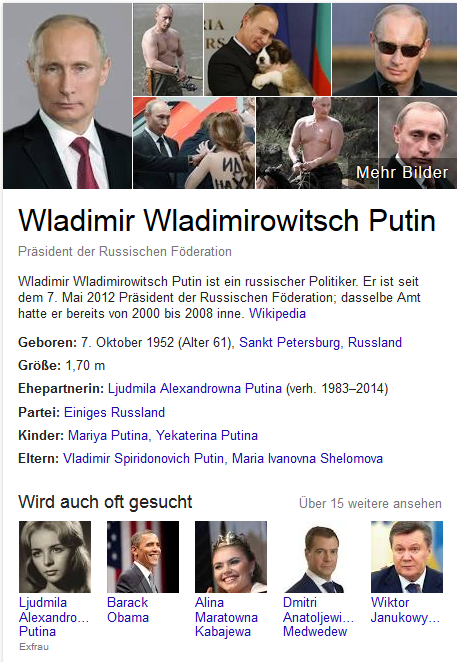
\includegraphics[scale=0.25]{img/putin_freebase.png}
\end{minipage}
\end{frame}

\begin{frame}
\frametitle{Concepts}
\begin{itemize}
  \item Topics = nodes of the graph (Bob Dylan, Mercedes, \ldots)
  \item Properties = edges of the graph (born in, produces, \ldots)
  \item Type (songwriter, actor, car, \ldots)
  \begin{itemize}
    \item Compound Value Types
   \end{itemize}
  \item Domain (music, business, \ldots)
  \item Hierarchical URIs (e.g.
  \url{http://www.freebase.com/} \\ \url{automotive/engine/horsepower})
\end{itemize}
\end{frame}

\begin{frame}
\frametitle{Access}
 Read
  \begin{itemize}
  \item RDF API
  \begin{itemize}
    \item  \url{http://rdf.freebase.com/ns/en.al_gore}
  \end{itemize}
  \item Search API (text search, ordered results after relevance)
  \begin{itemize}
    \item  \url{www.googleapis.com/freebase/v1/search?query=gore}
  \end{itemize}
  \item Topic API (get the JSON for a specific topic)
  \begin{itemize}
    \item  \url{www.googleapis.com/freebase/v1/topic/en/al_gore}
  \end{itemize}
  \item Data dumps
  \item Freebase Search Widget (jQuery plugin)
  \end{itemize}
  Read/Write
  \begin{itemize}
  \item MQL API
  \item Webpage (edit data, create views)
  \end{itemize}
  The Google APIs are available for Java, PHP, Python, .NET, JavaScript,
  Objective-C
\end{frame}

\begin{frame}[fragile]
\frametitle{Metaweb Query Language}
\begin{itemize}
  \item Read request sends and gets JSON
  \item[]
  \item
  \url{https://www.googleapis.com/freebase/v1/mqlread?query=\_jsonInput\_}\\
    \begin{verbatim}_jsonInput_:= {"type":"/music/artist",
  	            "name":"The Police",
  	            "album":[]}} 
\end{verbatim}
\end{itemize}
\end{frame}



\begin{frame}[fragile]
\frametitle{Metaweb Query Language}
\begin{itemize}
  \item Write request sends and gets JSON
  \item[]
  \item
  \url{https://www.googleapis.com/freebase/v1sandbox/mqlwrite?oauth_token=_token_&query=_query_}\\
    \begin{verbatim}_query_:= {"create":"unconditional",
		           "id":null,
		           "name":"Nowhere",
		           "type":"/location/location"} 
\end{verbatim}
\end{itemize}
\end{frame}